\section[Einleitung]{Einleitung}

\begin{sloppypar}  % Verhindert überlaufende Zeilen (nur bei Bedarf verwenden)
    In dieser Studie wird [...] Dichtefunktionaltheorie und Coupled Cluster verglichen.\footnote{Eine Fussnotiz kommt hier hin \textcite{Nicolaou}}
\end{sloppypar}

% ========================
%  UNTERABSCHNITT
% ========================
\subsection{Diels-Alder Reaktion}
Die Diels-Alder-Reaktion ist eine [...] in der synthetischen organischen Chemie.\autocite{Nicolaou} 

% ========================
%  MATHEMATISCHE GRUNDLAGEN
% ========================
Elektronischer Hamilton-Operator (\cref{eq:hamiltonian})
\begin{myequation}
    \hat{H}_{\text{el}} = -\frac{1}{2} \sum_{i=1}^N \nabla_i^2 
    - \sum_{i=1}^N \sum_{\alpha=1}^{M} \frac{Z_\alpha}{|\mathbf{r}_i - \mathbf{R}_\alpha|} 
    + \sum_{i > j}^N \frac{1}{|\mathbf{r}_i - \mathbf{r}_j|}
    \label{eq:hamiltonian}
\end{myequation}

% Slater-Determinante (Gleichung 2)
\begin{myequation}
    \tilde{\Psi}(\mathbf{r}_1, \dots, \mathbf{r}_N) = \frac{1}{\sqrt{N!}} 
    \begin{vmatrix}
    \phi_1(\mathbf{r}_1) & \cdots & \phi_1(\mathbf{r}_N) \\
    \vdots & \ddots & \vdots \\
    \phi_N(\mathbf{r}_1) & \cdots & \phi_N(\mathbf{r}_N)
    \end{vmatrix}
    \label{eq:slater}
\end{myequation}

% ========================
%  ABBILDUNG in Latex
% ========================

So kann man im Text auf die Abbildung verweisen: \cref{fig:scf}

\begin{abbfigure}[H]  % [H] erzwingt genaue Positionierung
    \centering
    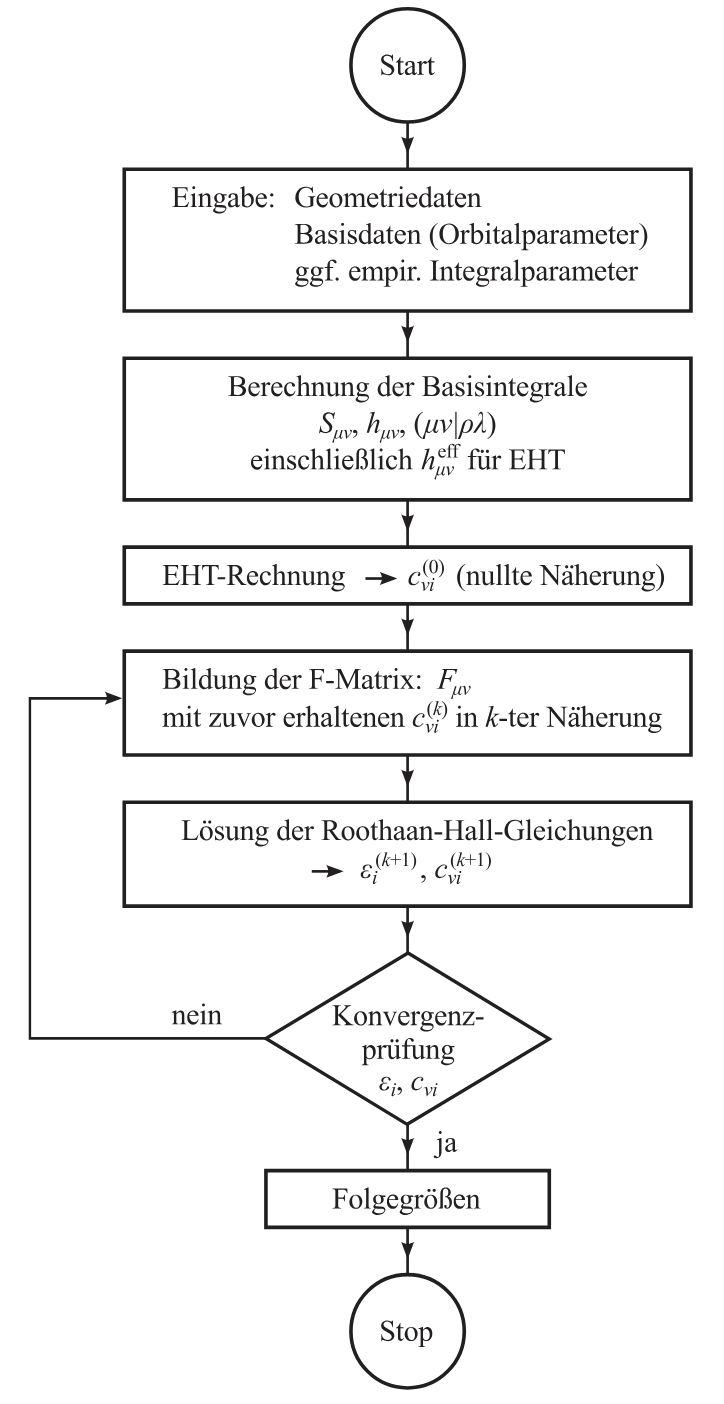
\includegraphics[width=.2\textwidth]{Graphik/SCF.png}
    \caption{Eine graphische Darstellung der SCF Methode.\autocite{Zülicke2015}}
    \label{fig:scf}
\end{abbfigure}

% ========================
%  Listen in Latex
% ========================
\begin{itemize}
    \item \textbf{Orbitale vom Gaußschen Typ (GTOs)}: 
    \begin{equation}
        \chi_\mu(\mathbf{r}) = N x^{l} y^{m} z^{n} e^{-\alpha \|\mathbf{r} - \mathbf{R}\|^2}
    \end{equation}
    \begin{tabular}{@{}ll@{}}
        \( N \): & Normierungskonstante \\
        \( \alpha \): & Exponent (radialer Zerfall) \\
        \( (l, m, n) \): & Drehimpulsquantenzahlen \\
        \( \mathbf{R} \): & Kernkoordinate \((X, Y, Z)\)
    \end{tabular}
    \autocite{Reinhold2015}

    \item \textbf{Slater-Type Orbitals (STOs)}: 
    \[ e^{-\zeta \|\mathbf{r} - \mathbf{R}\|} \]
    \begin{itemize}
        \item[+] Bessere Approximation der Atomorbitale
        \item[-] Rechenintensive Integralrechnung
        \item[→] Nur für spezielle Anwendungen/Referenzrechnungen
    \end{itemize}
    \autocite{Reinhold2015,Zülicke2015,Nicolaou}
\end{itemize}

% ========================
%  TABELLEN
% ========================
% Externe Tabellendateien einbinden
Auf diese kann man wie Abbildungen verweisen: \textbf{\cref{tab:geometrie}}

\begin{table}[H]
    \centering
    \caption{Die gemessenen Winkel und Abstände der optimierten Geometrien. Die farbigen Atome zeigen die zwischen denen die jeweilige Größe gemessenen wurde. Die blauen Atome sind von dem 2,5-Dioxo-2,5-dihydrofuran-3-carbonitril und die grünen sind von dem 2,3-Dichlorcyclopenta-1,3-dien.}
    \label{tab:geometrie}
    \resizebox{\textwidth}{!}{%
    \begin{tabular}{@{}l S[table-format=3.3] S[table-format=3.3] S[table-format=1.3] S[table-format=1.3]@{}}
    \toprule
                     & {Diederwinkel / \si{\degree}}        & {Winkel / \si{\degree}}     & \multicolumn{2}{c}{intramolekulare Distanz / \si{\angstrom}} \\ \midrule
                     & {\ch{O=}{\color[HTML]{0099FF}C}\ch{-}{\color[HTML]{0099FF}C}(CN)\ch{-}{\color[HTML]{0099FF}C}H\ch{-}{\color[HTML]{0099FF}C}\ch{=O}} 
                     & {H{\color[HTML]{00CC66}C}\ch{-}{\color[HTML]{00CC66}C}H\textsubscript{2}\ch{-}{\color[HTML]{00CC66}C}H} 
                     & {NC\ch{-}{\color[HTML]{0099FF}C}\ch{-}{\color[HTML]{00CC66}C}H}        
                     & {H{\color[HTML]{0099FF}C}\ch{-}{\color[HTML]{00CC66}C}H}               \\
    Präkomplex       & 179.635                            & 103.941                   & 3.171                          & 3.159                         \\
    Übergangszustand & 175.785                            & 99.973                    & 2.309                          & 2.038                         \\
    Produkt          & 177.903                            & 93.887                    & 1.590                          & 1.570                         \\ 
    \bottomrule
    \end{tabular}%
    }
\end{table}
\begin{table}[H]
    \caption{Die berechneten Energiedifferenzen in \unit{\kilo\joule\per\mole}.}
    \centering
    \begin{threeparttable}
    \label{tab:energie}
    \begin{tabular}{@{}l *{4}{S[table-format=-3.2]} @{}}
    \toprule
                                  & {DFT}         & {DFT + ZPE}    & {CC}          & {CC + ZPE}     \\
                                  & \multicolumn{4}{|c|}{\unit{\kilo\joule\per\mol}} \\ \midrule
    \makecell{Edukte - Präkomplex \\ (\textbf{Assoziationsenergie})}          &  -37.24        &  -34.02         &  -32.39        &  -29.17         \\
    \makecell{Edukte - Übergangszustand \\ (\textbf{Aktivierungsenergie})} & 16.40        & 23.07         & 20.78        & 27.45         \\
    \makecell{Edukte - Produkt \\ (\textbf{thermodynamische Energie}\textsuperscript{a})}             &  -90.75        &  -72.57         & -135.71        & -117.52         \\
    \bottomrule
    \end{tabular}
    
    \begin{tablenotes}
    \item[a] Auch als Reaktionsenthalpie \textDelta H bekannt, wird aber im weiteren Verlauf mit \textDelta E bezeichnet
    \end{tablenotes}
    \end{threeparttable}
\end{table}